%!TEX root = thesis.tex

\chapter{Visualisation Design}
\label{chap:visualisation-design}

Following the field study (see Chapter~\ref{chap:exploratory-field-study}), a strategy for visualisation prototyping and evaluation was developed. This process and the result are outlined in the following sections.

{\color{red}\cite{Ware2013a,McLean2010a,Purchase1996} will be useful here.}

\section{Rationale}


\section{Design}

\begin{figure}
  \centering 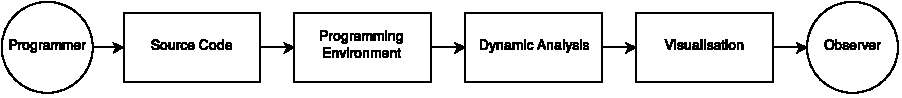
\includegraphics[width=\columnwidth]{../images/diagrams/knowledge-flow-initial.pdf}
  \caption{Knowledge flow from programmer to observer as directed by the visualisation technique employed.}
\label{fig:knowledge-flow-initial}
\end{figure}

\begin{figure}
\centering
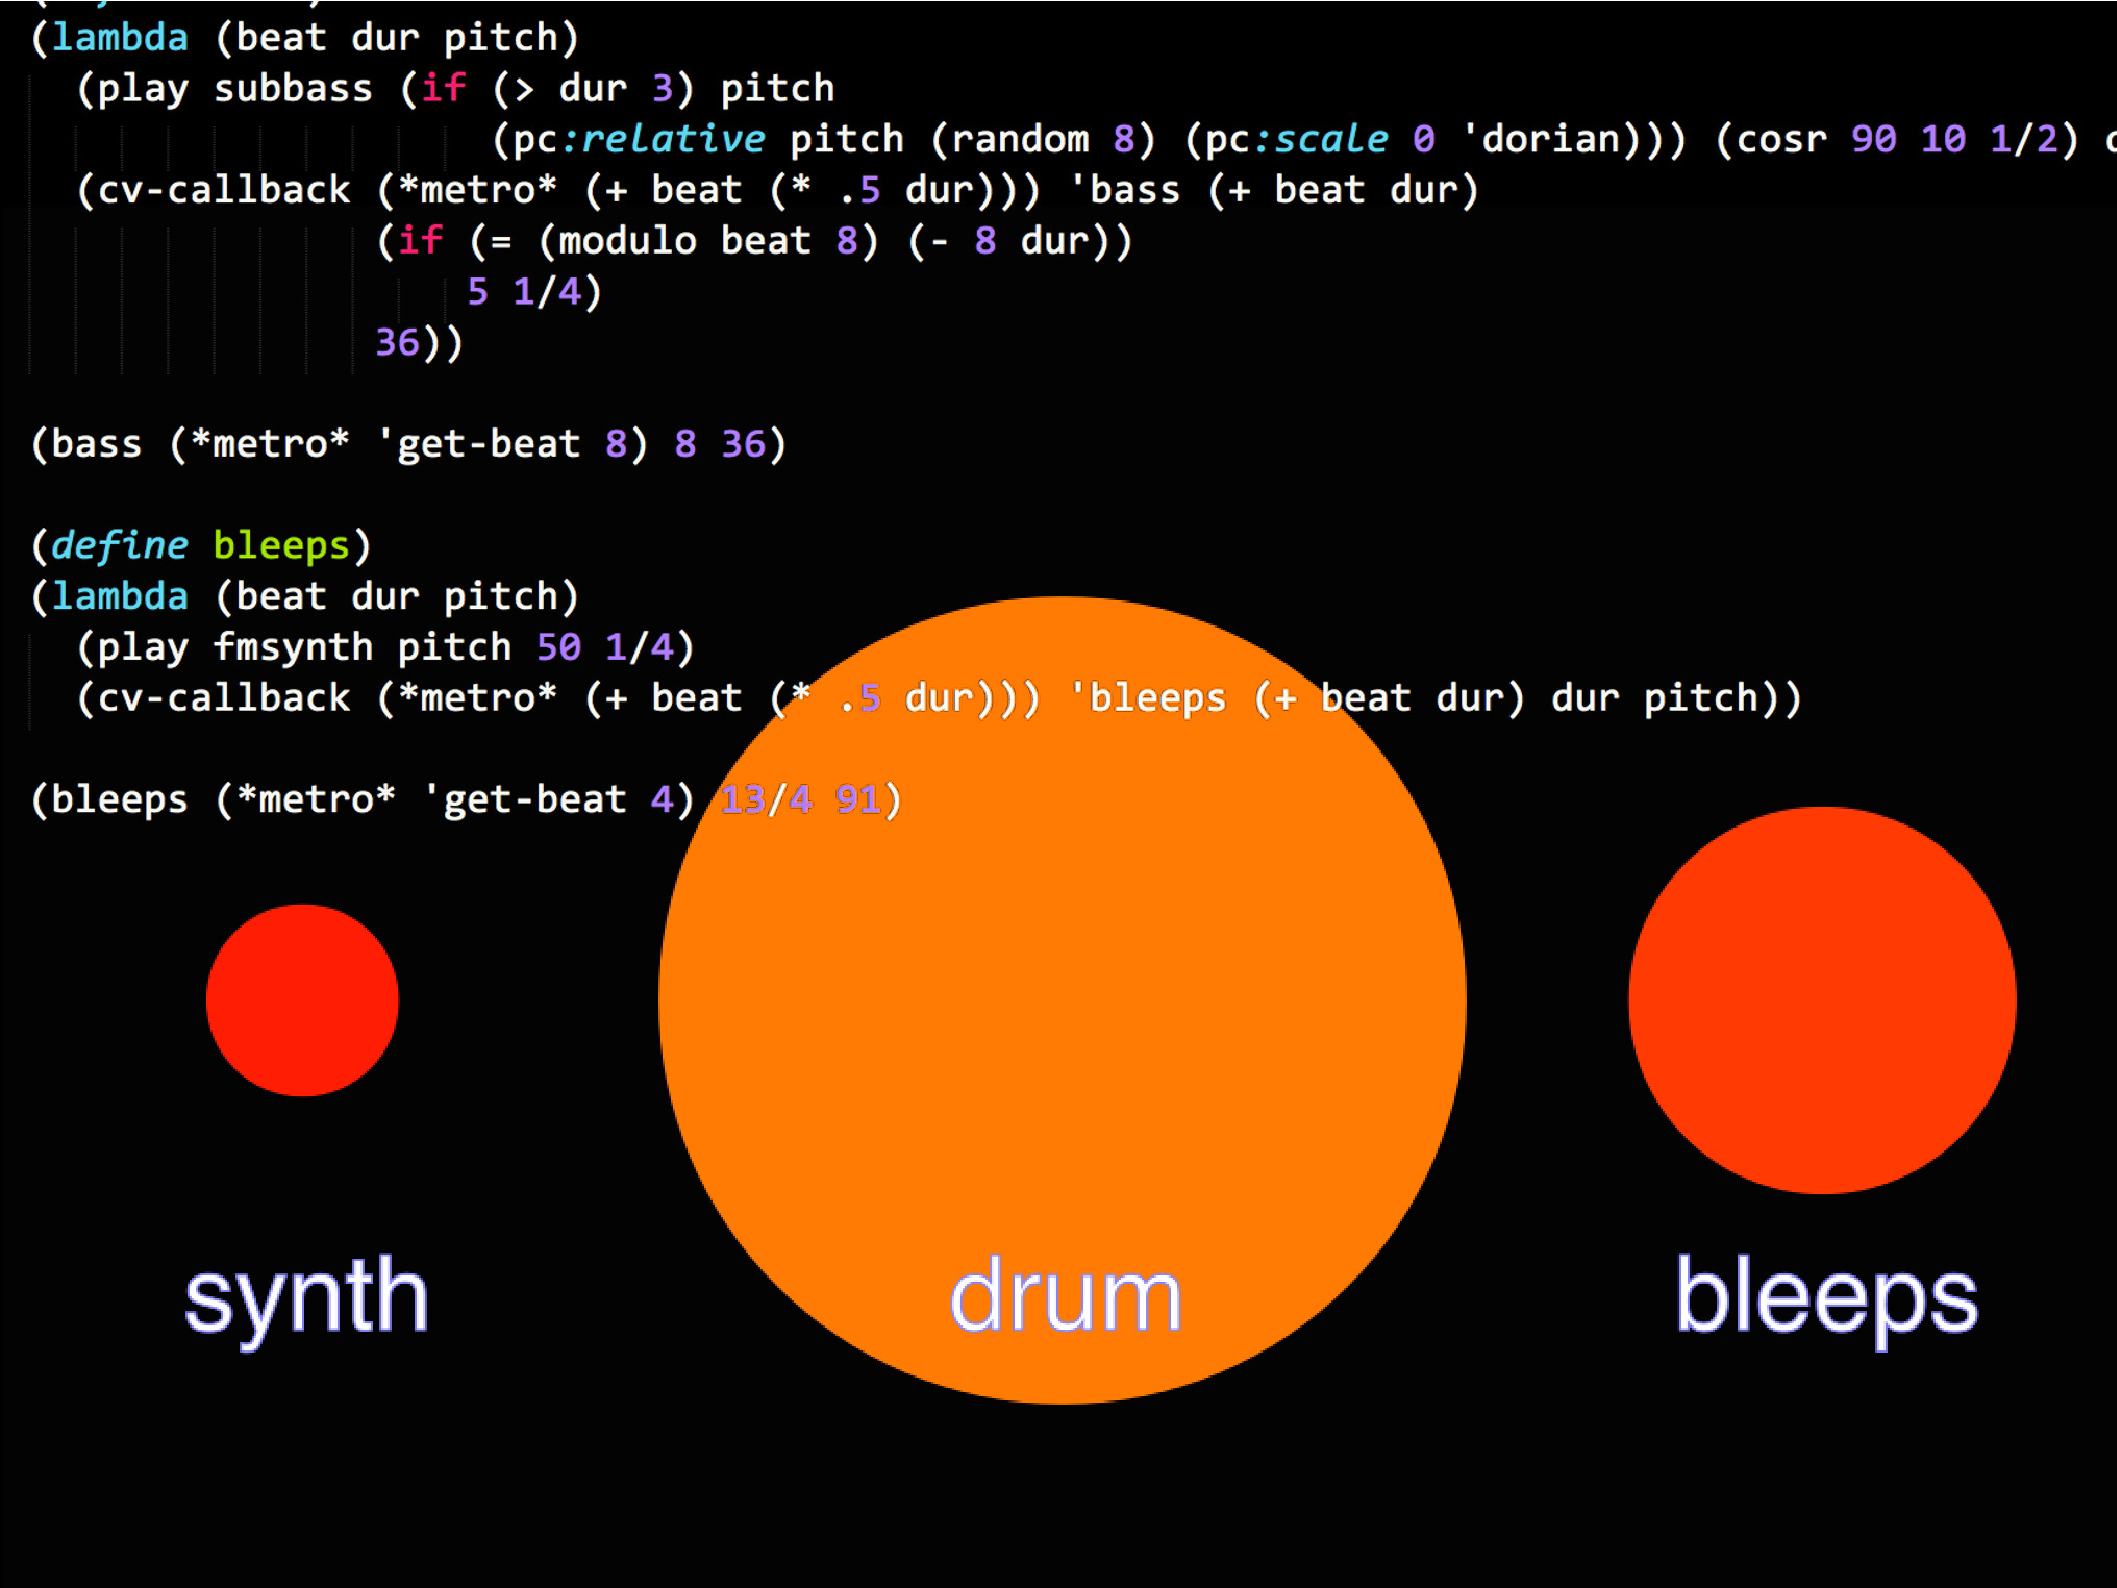
\includegraphics[width=0.75\columnwidth]{../study-2/results/visualisations/didactic-vis-overlay}
\caption{An example didactic visualisation.}
\label{fig:didactic-visualisation}
\end{figure}

\begin{figure}
\centering
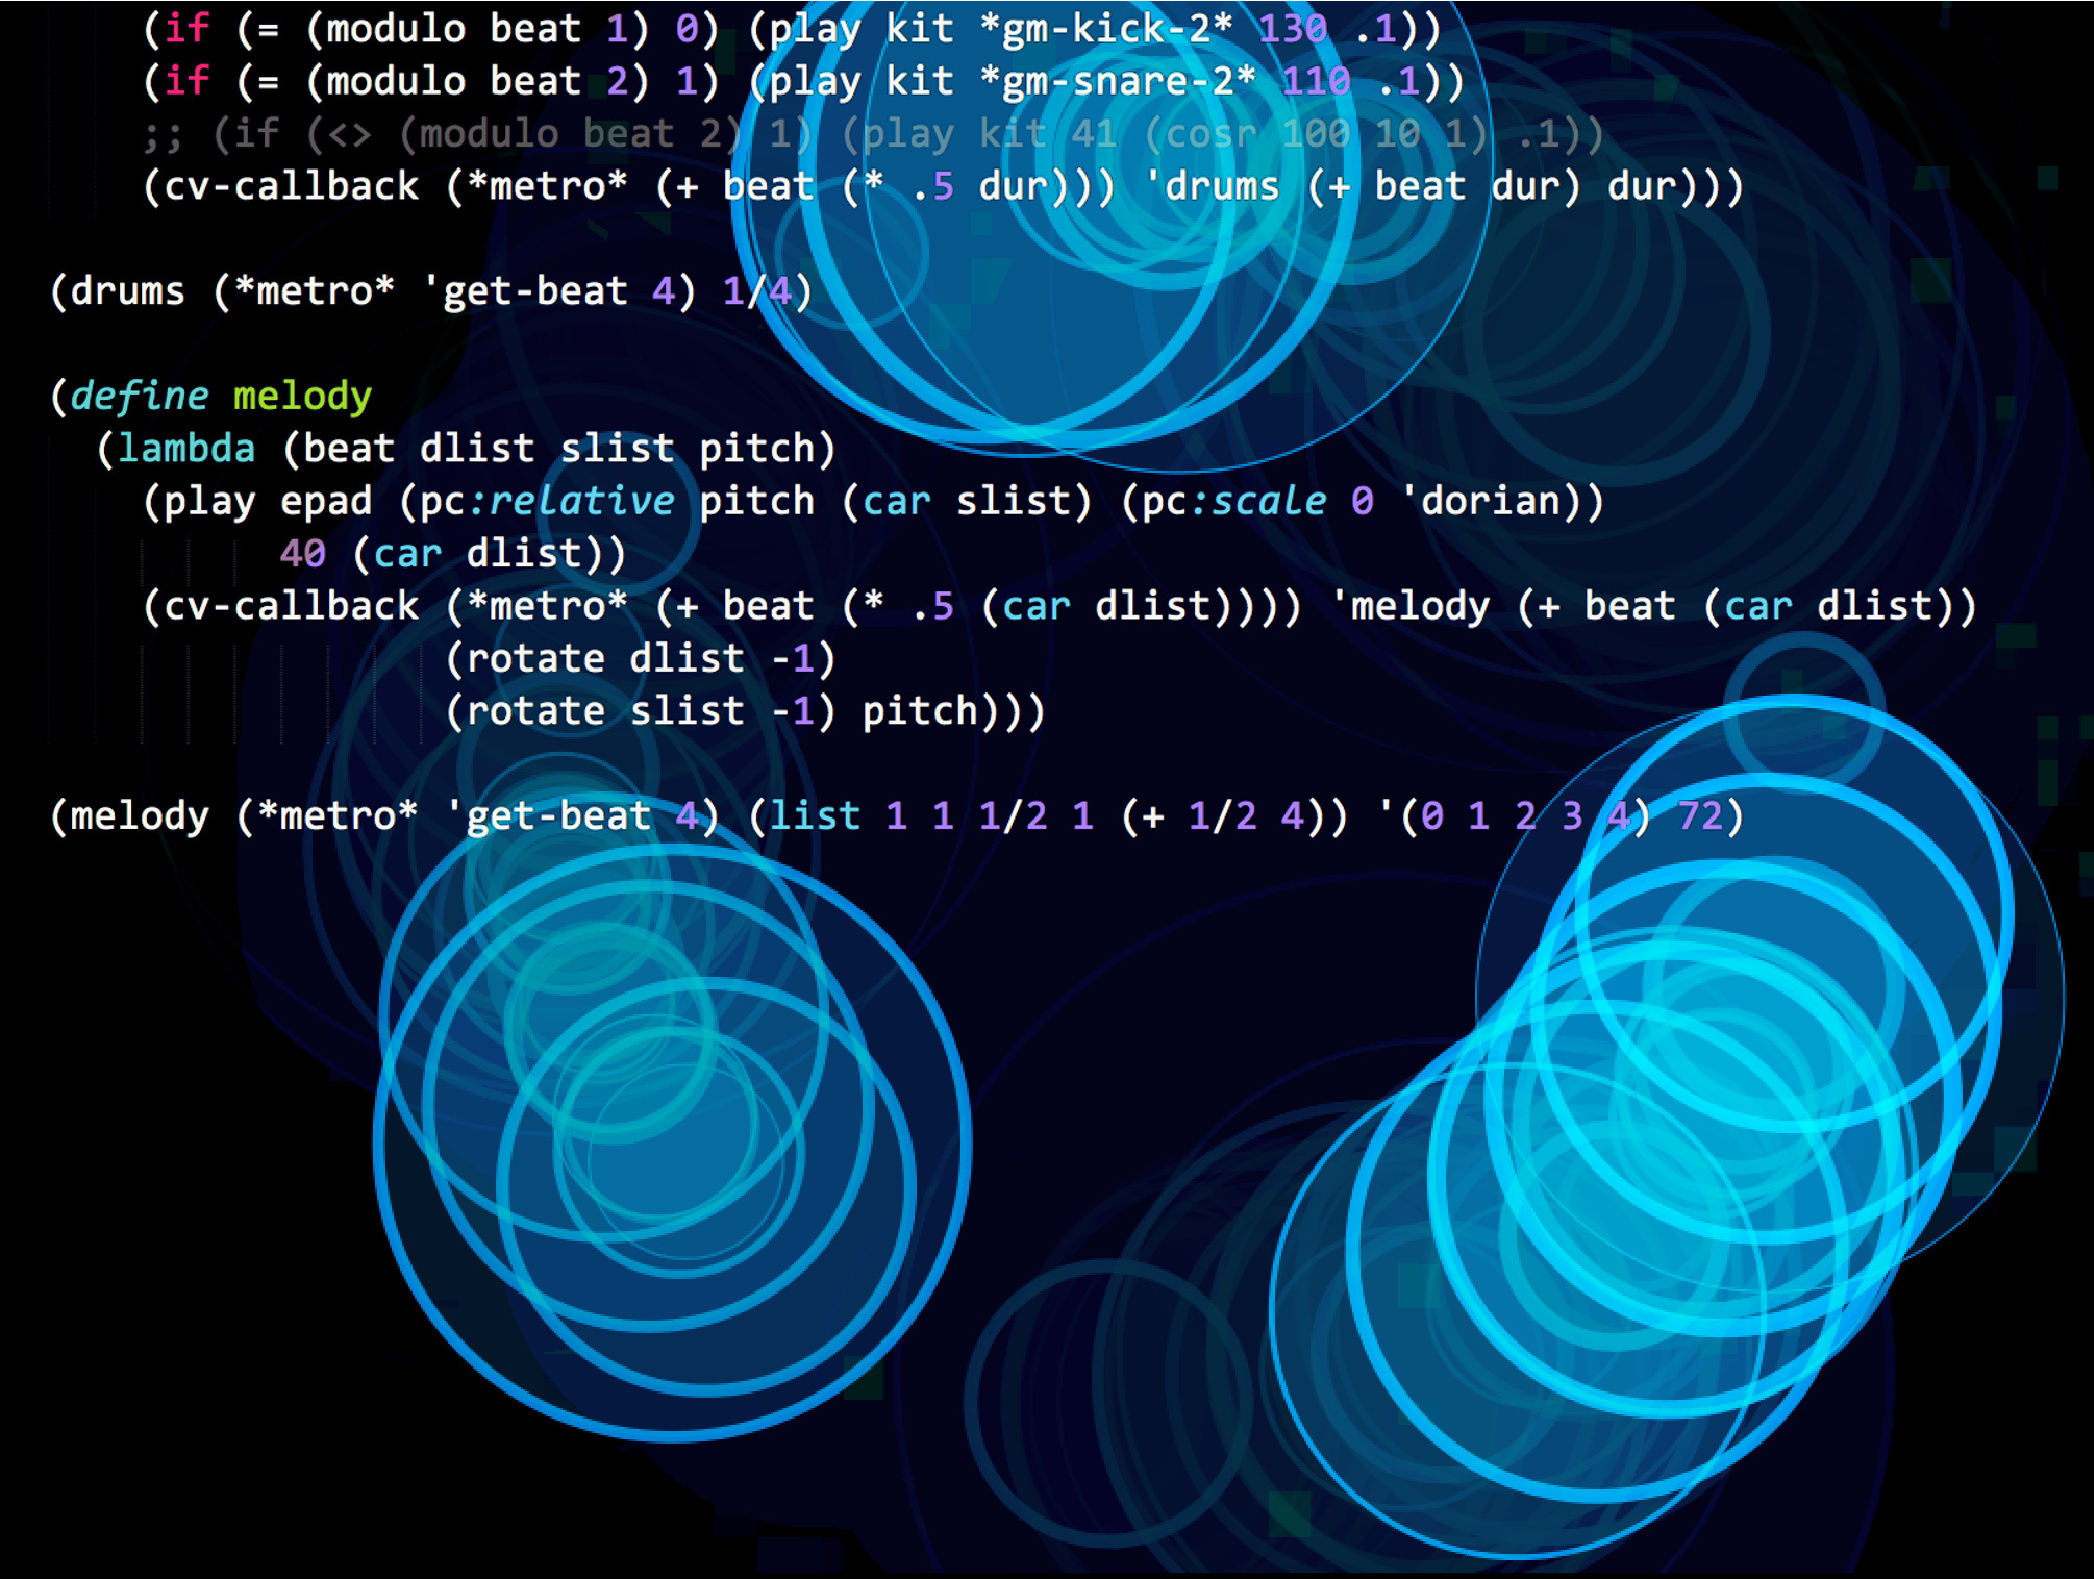
\includegraphics[width=0.75\columnwidth]{../study-2/results/visualisations/aesthetic-vis-overlay}
\caption{An example aesthetic visualisation.}
\label{fig:aesthetic-visualisation}
\end{figure}

Visualisations developed employed dynamic analysis of the running code to generate the visuals. The intended knowledge flow from programmer to observer is shown in Figure~\ref{fig:knowledge-flow-initial}.

Music visualisation is an extremely rich
and open-ended task, so to guide the development of the visualisations
for our lab study, we used the concepts of understanding and enjoyment
from the initial survey to develop two new code visualisations: a
\emph{didactic} one and an \emph{aesthetic} one.

\subsection{Didactic Visualisation}

The didactic visualisation (shown in
Figure~\ref{fig:didactic-visualisation}) attempted to communicate
\emph{information} about the actions of the programmer, prominently
displaying the \emph{names} of the active (source code) functions and
the ``time until next execution'' for each function (which is
particularly relevant in a time-sensitive programming context such as
music making). Bright colours and solid shapes were used to ensure
constant visibility and to communicate the intention of the underlying
code. The didactic visualisations proceeded through four stages, with
phase changes made depending on the number of active functions
(instruments).

\subsection{Aesthetic Visualisation}

The aesthetic visualisation technique was designed
to react to the programmer's activity in a more abstract way, to
maximise aesthetic appeal~\cite{Cawthon2007} and to engage the
audience's interest. Although still based on the source code and the
livecoder's edits, the generation of shapes was driven by instrument
volume and synchronised with the musical beat. The emphasis for the
aesthetic visualisation was on the artistic appeal of the visuals (see
Figure~\ref{fig:aesthetic-visualisation}), including more variety in
visual structure and colour. As in the didactic condition, the
aesthetic visualisations proceeded through four stages, based on the
number of active functions (instruments), but these visuals had no
textual labels and they moved and interacted with each other over the
entire projected scene.

\section{Mappings}


